\subsection{运行环境}
程序在以下环境下构建和测试.
\begin{description}
    \item[操作系统] macOS 13.1 22C5044e arm64;
    \item[c编译器] gcc (Homebrew GCC 12.2.0) 12.2.0;
    \item[构建和测试工具] GNU Make 3.81;
    \item[文档编译工具] XeTeX 3.141592653-2.6-0.999994 (TeX Live 2022)
    \item[文本编辑器] nvim v0.8.1
    \item[调试工具] Visual Studio Code Version: 1.74.0 (Universal)
\end{description}

\subsection{程序运行方式}
程序使用make进行构建. 读者优先程序和写者优先程序都会被构建在build/目录下.\par
对于程序的构建, 执行如下命令.
\begin{code}
    make
\end{code}

对于程序的执行, 可以使用如下命令:
\begin{code}
    Usage: build/[reader_priority | writer_priority] $(PEERS) $(RW_RATIO) $(SHM_SIZE)
\end{code}

其中, \$(PEERS)是将要创建的读者和写者进程总数, 建议不超过3000, 否则会导致操作系
统没有多余进程资源而导致操作系统不稳定. \$(RW\_RATIO)是读者和写者比例, 范围是0到
100. \$(SHM\_SIZE)是共享内存大小, 即创建多少个独立的共享内存块. 在本实验程序的实
现中, 对每个独立的共享内存块的访问进行独立控制.

\subsection{程序日志格式}
程序的日志有三种等级.\par

一级是最详细的日志, 包括进出关键区,进程创建和分化为读者写
者, 等待信号量耗时, 休眠时间和进程退出等信息, 随程序运行输出在标准输出中, 即
console中. 截取部分示例如下.\par
\begin{code}
    $ ./build/reader_priority 10 90 10

        [2022-12-16T15:48:41] Child with pid: 82474
        [2022-12-16T15:48:41] Child[82474](reader) accessing shared_memory[0].
    [2022-12-16T15:48:41] Child[82474](reader) waited for 0.000008 seconds.
        [2022-12-16T15:48:41] Sleep for 0.916291 seconds.
        [2022-12-16T15:48:41] Child with pid: 82477.
        [2022-12-16T15:48:41] Child with pid: 82475.
        [2022-12-16T15:48:41] Child[82475](reader) accessing shared_memory[9].
    [2022-12-16T15:48:41] Child[82477](reader) accessing shared_memory[7].
    [2022-12-16T15:48:41] Child[82475](reader) waited for 0.000018 seconds.
        [2022-12-16T15:48:41] Child[82477](reader) waited for 0.000028 seconds.
        [2022-12-16T15:48:41] Sleep for 1.609438 seconds.
        [2022-12-16T15:48:41] Sleep for -0.000000 seconds.
        [2022-12-16T15:48:41] Child[82475](reader) exited shared_memory[9].
    ...
\end{code}

二级是总结性日志, 在每个进程结束的时候写到logs/file.log文件中, 包括每个进程的读者和写者等待时间
总和, 以及读者和写者平均等待时间. 在日志的结尾还有对所有进程的读者和写者数量, 以
及运行次数判断统计. 此外, 每次输出日志的开头还会记录当前时间, 据此可以判断程序运
行时间. 由于通过宏定义的形式设定了每个进程运行LOOPS次后就会退出, 因此要展示稳定
运行20分钟以上的效果, 可以通过增加创建的子进程数量\$(PEERS)和减少能够访问的共享
内存块数量\$(SHM\_SIZE)来实现. 截取部分日志示例如下.\par

\begin{code}
    [2022-12-16T15:48:55] Child[82484]:
    Total write time: 0.000005 seconds; average write time: 0.000005 seconds.
    Total read time: 8.377258; average read time: 0.930806.
    Total time: 8.377263, total average time: 0.837726.

        [2022-12-16T15:48:57] Child[82474]:
    Total write time: 3.087316 seconds; average write time: 3.087316 seconds.
    Total read time: 7.399225; average read time: 0.822136.
    Total time: 10.486541, total average time: 1.048654.

        [2022-12-16T15:48:57] Child[82492]:
    Total write time: 0.000000 seconds; average write time: 0.000000 seconds.
    Total read time: 7.418502; average read time: 0.741850.
    Total time: 7.418502, total average time: 0.741850.


    VALIDATING RESULTS
    shared[0]: readers[9], writers[0]
    shared[1]: readers[11], writers[1]
    shared[2]: readers[5], writers[1]
    shared[3]: readers[7], writers[1]
    shared[4]: readers[9], writers[0]
    shared[5]: readers[8], writers[1]
    shared[6]: readers[11], writers[1]
    shared[7]: readers[15], writers[1]
    shared[8]: readers[10], writers[0]
    shared[9]: readers[8], writers[1]
    --------------------
    total: readers[93], writers[7]
    Total should be equal to (peers * LOOPS)[100]
    Result is right!

\end{code}

第三级日志很简略, 每次程序运行会追加一行到日志文件logs/stat.log的结尾, 分别为总
等待时间, 读者等待时间和写者等待时间. 用于多轮程序运行进行统计.


\subsection{运行结果}
分别采用读者优先策略和写者优先策略, 创建2000个读者写者, 读者比例50\%或90\%, 共享
内存块数量为10的情况下运行, 具体运行命令如下.
\begin{code}
    # Build
    make

    # 读者优先策略, 2000个读者写者, 50%读者, 10个共享内存块.
    build/reader_priority 2000 50 10

    # 读者优先策略, 2000个读者写者, 90%读者, 10个共享内存块.
    build/reader_priority 2000 90 10

    # 写者优先策略, 2000个读者写者, 50%读者, 10个共享内存块.
    build/writer_priority 2000 50 10

    # 写者优先策略, 2000个读者写者, 90%读者, 10个共享内存块.
    build/writer_priority 2000 90 10
\end{code}

得运行日志和读者/写者等待时间如下.
\begin{itemize}
    \item 读者优先策略, 读者比例50\%的运行日志为logs/50\_file\_reader\_priority.log,
          等待时间统计如图~\ref{fig:读者优先策略50}.
    \item 读者优先策略, 读者比例90\%的运行日志为logs/90\_file\_reader\_priority.log,
          等待时间统计如图~\ref{fig:读者优先策略90}.
    \item 写者优先策略, 读者比例50\%的运行日志为logs/50\_file\_reader\_priority.log,
          等待时间统计如图~\ref{fig:写者优先策略50}.
    \item 写者优先策略, 读者比例90\%的运行日志为logs/90\_file\_reader\_priority.log,
          等待时间统计如图~\ref{fig:写者优先策略90}.
\end{itemize}

\begin{figure}[ht!]
    \centering
    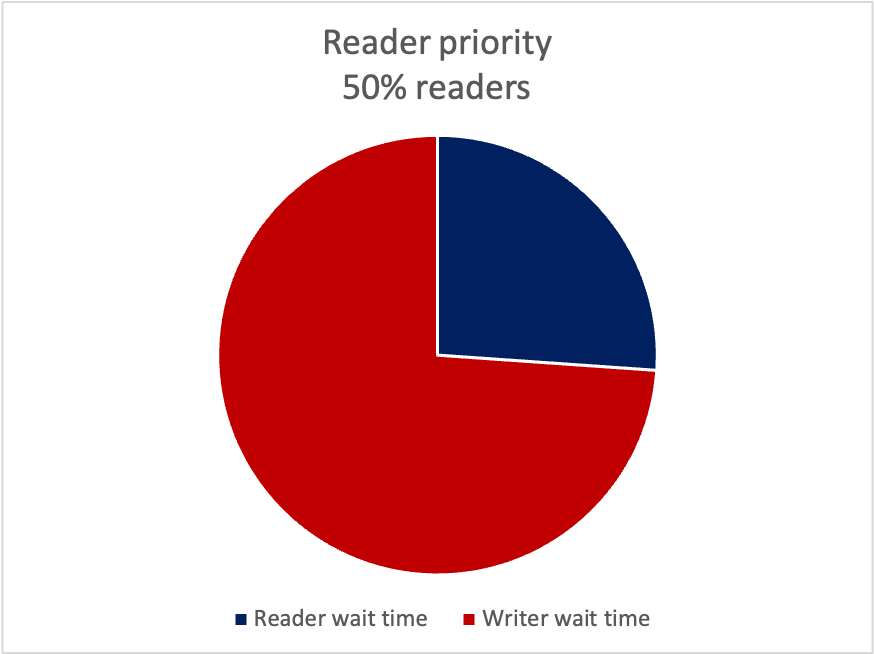
\includegraphics[width=0.95\textwidth]{50-reader-priority.png}
    \caption{读者优先策略,50\%读者}
    \label{fig:读者优先策略50}
\end{figure}
可以看到, 在均为50\%读者情况下, 读者优先策略和写者优先策略的表现是对称的, 即优先
的一方的等待时间占总等待时间的越$25\%$.
而均为90\%读者的情况下, 差异则比较大. 读者优先策略下, 读者和写者的等待时间大约对
半开, 而写者优先策略下, 几乎总是读者在等待, 而写者的等待时间相比之下很小. 可以预
见, 如果本实验程序中没有设置当进程访问LOOPS次共享内存后结束自己的话, 读者将几乎
不能访问共享内存.

\begin{figure}[ht!]
    \centering
    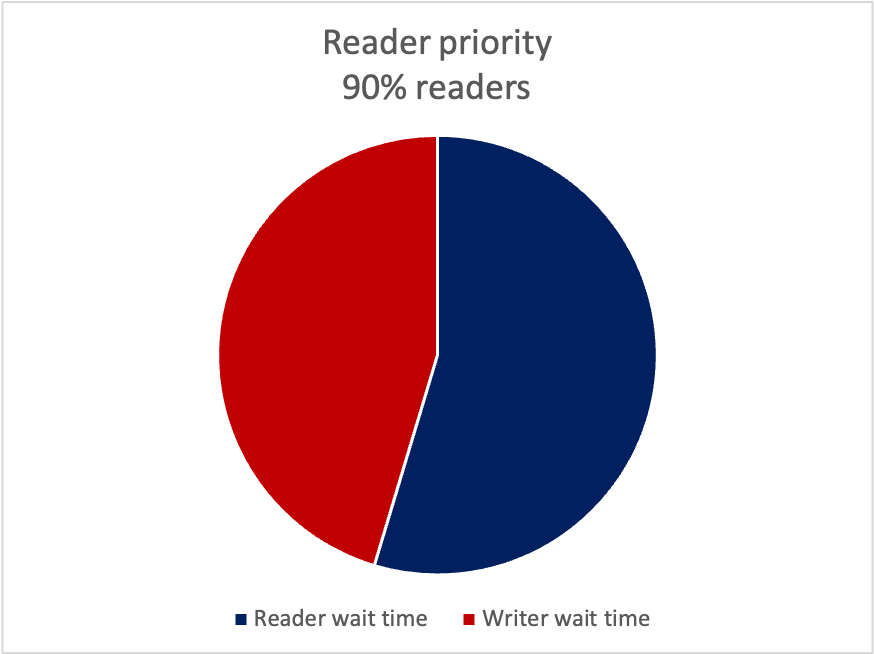
\includegraphics[width=0.95\textwidth]{90-reader-priority.png}
    \caption{读者优先策略,90\%读者}
    \label{fig:读者优先策略90}
\end{figure}

\begin{figure}[ht!]
    \centering
    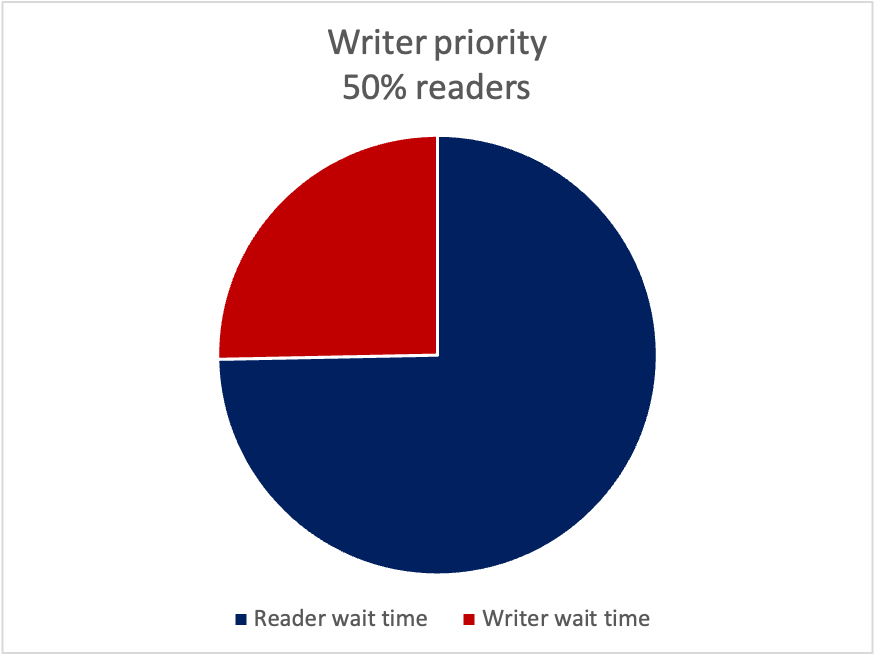
\includegraphics[width=0.95\textwidth]{50-writer-priority.png}
    \caption{写者优先策略,50\%读者}
    \label{fig:写者优先策略50}
\end{figure}

\begin{figure}[ht!]
    \centering
    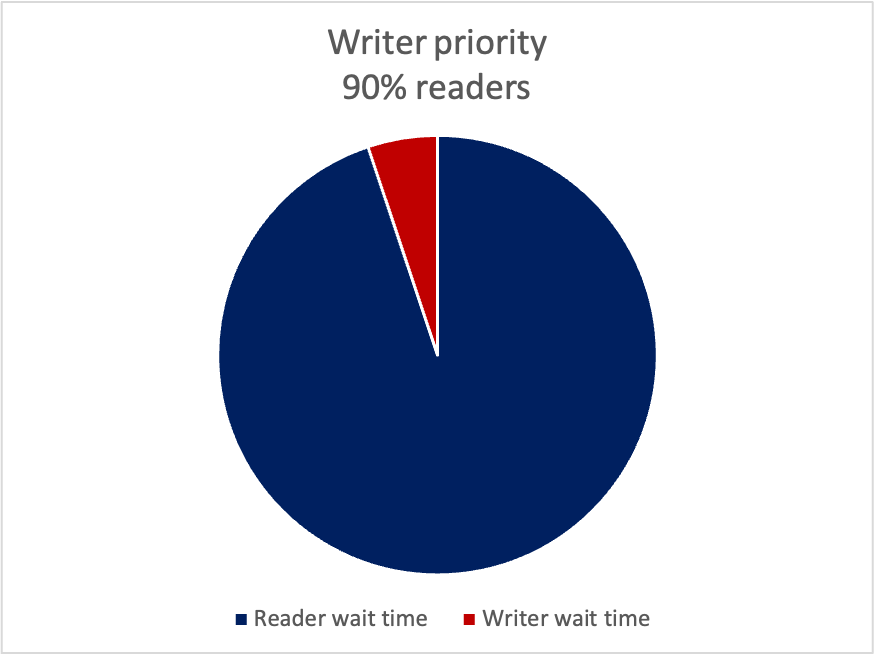
\includegraphics[width=0.95\textwidth]{90-writer-priority.png}
    \caption{写者优先策略,50\%读者}
    \label{fig:写者优先策略90}
\end{figure}